%!TEX root = ../../thesis.tex

The first theory of weak interactions was a four-point interaction with Fermi coupling 
constant \unit{$G_{\text{F}} = 1.166\times 10^{-5}$}{\GeV\rpsquared}. Although successful 
in describing low energy phenomena, such as nuclear $\beta$-decay and muon decay, at 
energies above \unit{\about300}{\GeV} the theory predicted cross sections which violate 
unitarity \cite{Aitchison}.

The solution was to introduce charged vector bosons (\PWpm bosons) to mediate the weak 
interaction, similar to the exchange of photons in QED. However, unlike QED, 
the weak interaction is short ranged and therefore its exchange bosons must be massive. 
Since the propagator for a particle of mass $m$ and momentum $p$ contains a factor 
$1 / (p^2 - m^2)$, in the low energy limit we can relate to Fermi's theory and identify 
that $G_{\text{F}} \sim g^2 / m_{\PW}^2$, where $g$ is the coupling of the vector boson. 
Thus, at low energies, the strength of the weak interaction is suppressed by the mass of the 
exchange boson.

At this time, there were two key obstacles to unifying the electromagnetic and weak 
interactions. First, the discovery of parity violation in cobalt-60 $\beta$-decay 
implied the weak interaction has a \VminusA structure, whereas QED has a pure V 
structure \cite{Wu:1957}.\footnote{
	Five bilinear covariants can be constructed from the Dirac $\gamma$ matrices, which 
	are named according to how they transform under parity: scalar, pseudoscalar, vector, 
	axial vector and tensor.
}
Second, the \PWpm bosons are massive whilst photons are massless. This was a major 
problem because gauge bosons are inherently massless.\footnote{
	Consider the gauge transformation of a Yang-Mills gauge field 
	$\bvec{W}_{\mu} \rightarrow \bvec{W}_{\mu} - \partial_{\mu} \bvec{\alpha}(x)
	- g \lbrack \bvec{\alpha}(x) \times \bvec{W}_{\mu} \rbrack$. Clearly the mass term 
	$-\tfrac{1}{2}m^2 \bvec{W}_{\mu} \cdot \bvec{W}^{\mu}$ is not gauge invariant, and 
	hence the gauge boson is massless.}
In fact, fermion masses were also forbidden by the chiral nature of the weak interaction, 
but were known to exist.\footnote{
	Consider a spinor as the sum of its left- and right-handed chiral states 
	$\psi = \psi_{\text{L}} + \psi_{\text{R}}$. Then the Dirac mass term is 
	$-m \bar{\psi} \psi = -m (\bar{\psi}_{\text{R}} \psi_{\text{L}} + 
	\bar{\psi}_{\text{L}} \psi_{\text{R}})$. For a chiral theory, $\psi_{\text{L}}$ and
	$\psi_{\text{R}}$ behave differently under gauge transformations and thus the mass 
	term is not gauge invariant.
}

Glashow's proposal of an \EWgroup group was a major step forward \cite{Glashow:1961}. 
This model describes three gauge fields \rowthreevec{W^1_{\mu}}{W^2_{\mu}}{W^3_{\mu}} 
which couple to weak isospin $T$ with strength $g$, and a single gauge field $B_{\mu}$ 
which couples to weak hypercharge $Y$ with strength $g'$. The subscript L indicates 
that only left-handed chiral particles couple to the $W^i_{\mu}$ fields, explaining the 
\VminusA nature of the weak interaction whilst preserving QED. The physical gauge 
fields are obtained through the mixing of these fields
\begin{align}
	W^{\pm}_{\mu} &= (W^1_{\mu} \mp i W^2_{\mu}) / \sqrt{2} \label{eq:Wfield} \\
	Z_{\mu} &= \cos\thetaW W^3_{\mu} - \sin\thetaW B_{\mu} \label{eq:Zfield} \\
	A_{\mu} &= \sin\thetaW W^3_{\mu} + \cos\thetaW B_{\mu} \label{eq:Afield}
\end{align}
where
\begin{equation}
	\cos\thetaW = g/\sqrt{g^2 + g'^2}
	\quad\quad \text{and} \quad\quad
	\sin\thetaW = g'/\sqrt{g^2 + g'^2} \,. 
	\label{eq:weak_mixing}
\end{equation}
We identify $W^{\pm}_{\mu}$ with the \PWpm bosons, $A_{\mu}$ with the photon 
and $Z_{\mu}$ with a new neutral \PZ boson. Weak neutral currents were later confirmed 
experimentally \cite{Gargamelle:1973}. 

\begin{table}[t]
	\begin{tabular}{ccc@{\hskip 1cm}cccc}
		\toprule
		& & & $T$ & $T_3$ & $Y$ & $Q$ \\
		\midrule
		\multirow{2}{*}{$\colvector{\Pnue\\ \Pe}_{\!\!\!\text{L}}$} & 
		\multirow{2}{*}{$\colvector{\Pnum\\ \Pmu}_{\!\!\!\text{L}}$} & 
		\multirow{2}{*}{$\colvector{\Pnut\\ \Ptau}_{\!\!\!\text{L}}$} & 
		$\tfrac{1}{2}$ & $+\tfrac{1}{2}$ & $-1$ & 0 \\
		& & & $\tfrac{1}{2}$ & $-\tfrac{1}{2}$ & $-1$ & $-1$ \\
		$\Pnue_{\text{R}}$ & $\Pnum_{\text{R}}$ & $\Pnut_{\text{R}}$ & 0 & 0 & 0 & 0 \\
		$\Pe_{\text{R}}$ & $\Pmu_{\text{R}}$ & $\Ptau_{\text{R}}$ & 0 & 0 & $-2$ & $-1$ \\
		\midrule
		\multirow{2}{*}{$\colvector{\Pup\\ \Pdown'}_{\!\!\!\text{L}}$} & 
		\multirow{2}{*}{$\colvector{\Pcharm\\ \Pstrange'}_{\!\!\!\text{L}}$} & 
		\multirow{2}{*}{$\colvector{\Ptop\\ \Pbottom'}_{\!\!\!\text{L}}$} & 
		$\tfrac{1}{2}$ & $+\tfrac{1}{2}$ & $+\tfrac{1}{3}$ & $+\tfrac{2}{3}$ \\
		& & & $\tfrac{1}{2}$ & $-\tfrac{1}{2}$ & $+\tfrac{1}{3}$ & $-\tfrac{1}{3}$ \\
		$\Pup_{\text{R}}$ & $\Pcharm_{\text{R}}$ & $\Ptop_{\text{R}}$ & 0 & 0 & $+\tfrac{4}{3}$ & $+\tfrac{2}{3}$ \\
		$\Pdown_{\text{R}}$ & $\Pstrange_{\text{R}}$ & $\Pbottom_{\text{R}}$ & 0 & 0 & $-\tfrac{2}{3}$ & $-\tfrac{1}{3}$ \\
		\bottomrule
	\end{tabular}
	\caption{The weak isospin $T$, weak hypercharge $Y$ and electric charge $Q$ of the 
	fermions. In charged currents, the states that couple to \Pup-type 
	quarks are superpositions of \Pdown-type quarks and are denoted with a prime. 
	Although right-handed neutrinos are decoupled, recent observations of neutrino 
	oscillations suggest these might exist.}
	\label{tab:ew_fermions}
\end{table}

Glashow's \EWgroup theory therefore predicts the interaction of fermions, in left-handed 
\SUgroup{2} doublets and right-handed \SUgroup{2} singlets (see 
\Table~\ref{tab:ew_fermions}), with \PWpm, \PZ and \Pphoton 
exchange bosons. Gauge boson self-interactions are also expected due to the non-abelian 
nature of the EW theory. The \PWpm bosons couple to weak isospin $T$ with strength 
$g$, the \PZ boson couples vectorially to $c_{\text{V}}$ and axially to $c_{\text{A}}$ 
with strength $g/(2\cos\thetaW)$, and the photon couples to electric charge $Q$ with 
strength $e = g\sin\thetaW$, where
\begin{align}
	c_{\text{V}} &= T_3 - 2 Q \sin^2\thetaW \,,\quad\quad c_{\text{A}} = T_3 \\
	Q   &= T_3 + \frac{Y}{2} \,.
\end{align}

Unfortunately, it was necessary to explicitly break the symmetry by adding mass terms for 
the \PWpm and \PZ bosons by hand. Initial attempts to invoke a mechanism of spontaneous 
symmetry breaking (SSB) were hindered by the Goldstone theorem.



\subsection{The Goldstone theorem}
\label{sec:ewsb:goldstone}

\begin{figure}[t]
	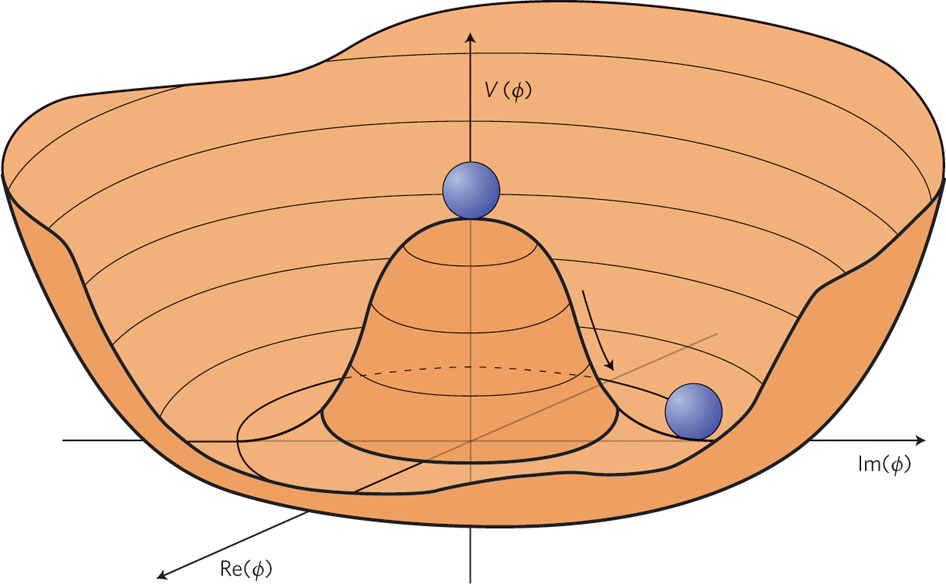
\includegraphics[width=\mediumfigwidth]{tex/motivation/sombrero}
	\caption{The sombrero potential, in which a vacuum state must be arbitrarily chosen, 
	spontaneously breaking the symmetry of the underlying Lagrangian.
	Fluctuations in the azimuthal direction correspond to a massless Nambu-Goldstone 
	boson. Fluctuations in the radial direction correspond to a massive Higgs boson.}
	\label{fig:sombrero}
\end{figure}

SSB arises when the vacuum state does not respect the symmetry in question. This can 
occur when a field acquires a non-zero vacuum expectation value. To see this, consider a 
complex scalar field $\phi$ described by the Lagrangian
\begin{equation}
	\mathcal{L} 
	= \parenths{\partial_{\mu}\phi^{\dagger}} \parenths{\partial^{\mu}\phi} 
	+ \mu^2 \phi^{\dagger}\phi - \lambda \parenths{\phi^{\dagger}\phi}^2
	\label{eq:lagr:goldstone}
\end{equation}
with positive $\mu^2$ and $\lambda$, giving a sombrero potential 
(\Figure~\ref{fig:sombrero}). 
Although $\mathcal{L}$ is invariant under global \Ugroup{1} transformations 
$\phi \rightarrow \eexp{-i\alpha} \phi$, there are infinite degenerate vacua
$\phi = \mu\eexp{-i\theta}/\sqrt{2\lambda}$ that are not invariant. In order to interact 
with the system, a single vacuum must be arbitrarily chosen, spontaneously breaking the 
\Ugroup{1} symmetry.

The Goldstone theorem states that SSB of a continuous global symmetry will lead to 
the existence of a number of massless scalar Nambu-Goldstone bosons \cite{Goldstone:1962}.
This can be seen by considering radial and azimuthal excitations, $h\parenths{x}$ and 
$\theta\parenths{x}$, about the vacuum 
\begin{equation}
	\phi\parenths{x} = \frac{1}{\sqrt{2}} \sqbracs{v + h\parenths{x}} \eexp{-i\theta\parenths{x} / v}
\end{equation}
where $v = \mu/\sqrt{\lambda}$. When substituted into (\ref{eq:lagr:goldstone}), we get
\begin{equation}
	\mathcal{L} = \tfrac{1}{2}\partial_{\mu}\theta \partial^{\mu}\theta
	+ \tfrac{1}{2}\partial_{\mu}h \partial^{\mu}h
	- \mu^2 h^2
	+ \dots
\end{equation}
where the dots denote terms neither kinetic nor mass. 
We identify a massless Nambu-Goldstone boson (the $\theta$-mode) and a Higgs boson of 
mass $\sqrt{2}\mu$ (the $h$-mode).

In order to explain massive \PWpm and \PZ bosons, the electroweak symmetry must be broken.
But the Goldstone theorem suggested that this would predict massless scalar bosons, which
were not experimentally observed.



\subsection{The Higgs mechanism}
\label{sec:ewsb:higgs}

However, when SSB of a continuous \textit{local} symmetry is studied, something 
remarkable happens. The Nambu-Goldstone bosons of the theory are `eaten' by the gauge 
bosons, giving them mass. The associated degrees of freedom appear as longitudinal 
components of the massive gauge bosons. This is known as the Higgs mechanism 
\cite{Englert:1964,Higgs:1964a,Higgs:1964b,Guralnik:1964,Higgs:1966}.

Consider the Lagrangian for a \Ugroup{1} gauge theory with a sombrero potential
\begin{equation}
	\mathcal{L} 
	= \parenths{D_{\mu}\phi}^{\dagger} \parenths{D^{\mu}\phi}
	- \tfrac{1}{4} F_{\mu\nu} F^{\mu\nu}
	+ \mu^2 \phi^{\dagger} \phi - \lambda \parenths{\phi^{\dagger} \phi}^2
	\label{eq:lagr:abelHiggs}
\end{equation}
where $D_{\mu} = \partial_{\mu} + iqA_{\mu}$ is the covariant derivative and $F_{\mu\nu} 
= \partial_{\mu}A_{\nu} - \partial_{\nu}A_{\mu}$ is the field tensor. This is invariant 
under local \Ugroup{1} transformations $\phi \rightarrow \eexp{-i\alpha\parenths{x}} \phi$
when accompanied by a gauge transformation of the potential 
$A_{\mu} \rightarrow A_{\mu} + \tfrac{1}{q}\partial_{\mu} \alpha\parenths{x}$.

We are free to choose the unitary gauge $\alpha\parenths{x} = -\theta\parenths{x}/v$,
absorbing the $\theta$-mode into the photon field 
$A_{\mu} \rightarrow A_{\mu} - \tfrac{1}{qv}\partial_{\mu} \theta\parenths{x}$. 
Ultimately, the final result is gauge-independent, but other choices require the 
Nambu-Goldstone bosons to be explicitly included in the Feynman rules. Since the 
$\theta$-mode is `gauged away', excitations about the vacuum become
\begin{equation}
	\phi\parenths{x} = \frac{1}{\sqrt{2}} \sqbracs{v + h\parenths{x}}
\end{equation}
and the Lagrangian (\ref{eq:lagr:abelHiggs}) becomes
\begin{equation}
	\mathcal{L}
	= \tfrac{1}{2} q^2 v^2 A_{\mu} A^{\mu}
	- \tfrac{1}{4} F_{\mu\nu}F^{\mu\nu}
	+ \tfrac{1}{2} \partial_{\mu}h \partial^{\mu}h
	- \mu^2 h^2
	+ \dots
\end{equation}
where the dots denote terms neither kinetic nor mass. 
The Nambu-Goldstone boson is no longer present and the photon has acquired a mass $qv$.
Again, there is a massive scalar Higgs boson as a by-product of the SSB.



\subsection{Glashow-Salam-Weinberg electroweak theory}

The Higgs mechanism can be extended to non-abelian gauge theories, as was necessary to 
describe electroweak symmetry breaking \cite{Kibble:1967,Weinberg:1967,Salam:1968}.
Consider the Lagrangian for an $\SUgroup{2}\times\Ugroup{1}$ gauge theory with a sombrero
potential
\begin{equation}
	\mathcal{L} 
	= \parenths{D_{\mu}\phi}^{\dagger} \parenths{D^{\mu}\phi}
	- \tfrac{1}{4} \bvec{F}_{\mu\nu} \cdot \bvec{F}^{\mu\nu}
	- \tfrac{1}{4} G_{\mu\nu} G^{\mu\nu}
	+ \mu^2 \phi^{\dagger} \phi - \lambda \parenths{\phi^{\dagger} \phi}^2
	\label{eq:lagr:ewHiggs}
\end{equation}
where $D_{\mu} = \partial_{\mu} + \tfrac{i}{2} g \bvec{\tau} \cdot \bvec{W}_{\mu} + 
\tfrac{i}{2} g' Y B_{\mu}$ is the covariant derivative, and $\bvec{F}_{\mu\nu} = 
\partial_{\mu}\bvec{W}_{\nu} - \partial_{\nu}\bvec{W}_{\mu} - g \bvec{W}_{\mu} \cross 
\bvec{W}_{\nu}$ and $G_{\mu\nu} = \partial_{\mu}B_{\nu} - \partial_{\nu}B_{\mu}$ are the
field tensors. In this case, $\phi$ is an \SUgroup{2} doublet of complex scalar fields
\begin{equation}
	\phi = \colvector{\phi^+\\\phi^0} = \frac{1}{\sqrt{2}} \colvector{ \phi_1 + i\phi_2\\ \phi_3 + i\phi_4}.
\end{equation}

Again, there are infinite degenerate vacua satisfying 
$\parenths{\phi_1^2 + \phi_2^2 + \phi_3^2 + \phi_4^2} = \mu^2/\lambda$. In analogue with 
the abelian Higgs mechanism, the unitary gauge absorbs the $\phi_1$, $\phi_2$ and 
$\phi_4$-modes into the gauge fields. Thus, considering excitations about the vacuum
\begin{equation}
	\phi\parenths{x} = \frac{1}{\sqrt{2}} \colvector{0\\  
	v + h\parenths{x}} \label{eq:higgs_doublet}
\end{equation}
the Lagrangian (\ref{eq:lagr:ewHiggs}) becomes
\begin{align}
	\mathcal{L} &= \tfrac{1}{8} g^2 v^2 \bvec{W}_{\mu} \cdot \bvec{W}^{\mu} - \tfrac{1}{4} \bvec{F}_{\mu\nu} \cdot \bvec{F}^{\mu\nu} + \tfrac{1}{8} v^2 g'^2 B_{\mu} B^{\mu} - \tfrac{1}{4} v^2 gg' B_{\mu} W_{3}^{\mu} - \tfrac{1}{4} G_{\mu\nu} G^{\mu\nu} \nonumber \\
	&\quad\quad {} + \tfrac{1}{2} \partial_{\mu}h \partial^{\mu}h - \mu^2 h^2 + \dots \\
	&= \tfrac{1}{4} g^2 v^2 W^{+}_{\mu} W^{-\mu} - \tfrac{1}{2} \parenths{\partial_{\mu}W^{+}_{\nu} - \partial_{\nu}W^{+}_{\mu}} \parenths{\partial^{\mu}W^{-\nu} - \partial^{\nu}W^{-\mu}} \nonumber \\
	&\quad\quad {} + \tfrac{1}{8} v^2 \parenths{g^2 + g'^2} Z_{\mu} Z^{\mu} - \tfrac{1}{4} \parenths{\partial_{\mu}Z_{\nu} - \partial_{\nu}Z_{\mu}} \parenths{\partial^{\mu}Z^{\nu} - \partial^{\nu}Z^{\mu}} - \tfrac{1}{4} F_{\mu\nu} F^{\mu\nu} \nonumber \\
	&\quad\quad {} + \tfrac{1}{2} \partial_{\mu}h \partial^{\mu}h - \mu^2 h^2 + \dots
\end{align}
where the dots denote terms neither kinetic nor mass, $F_{\mu\nu}$ is the field tensor of
QED, and the expression has been rewritten in terms of the physical gauge fields 
using (\ref{eq:Wfield}), (\ref{eq:Zfield}) and (\ref{eq:Afield}). The \PWpm bosons 
acquire a mass $gv/2$ and the \PZ boson acquires a mass $v \sqrt{\parenths{g^2+g'^2}}/2$, 
while the photon is massless. Again, all Nambu-Goldstone bosons are gone and a Higgs 
boson has appeared as a by-product of the SSB.

This theory predicts a striking relation between the gauge boson masses, using 
(\ref{eq:weak_mixing})
\begin{equation}
	\mW = \mZ \cos\thetaW
\end{equation}
which was experimentally verified once the \PW and \PZ bosons were discovered 
\cite{UA1:Wboson,UA2:Wboson,UA1:Zboson,UA2:Zboson,UA1:1989}. It also predicted a massive 
scalar Higgs boson, whose mass could not be determined from the other parameters of the 
theory.

Fermion masses can also be incorporated into EW theory through Yukawa couplings.
Consider a coupling between the electron-type \SUgroup{2} doublet (see 
\Table~\ref{tab:ew_fermions}), the Higgs doublet $\phi$ given in 
(\ref{eq:higgs_doublet}), and the electron \SUgroup{2} singlet
\begin{align}
	\mathcal{L}_{\Pe}^{\text{Yuk}} &= -g_{\Pe} \parenths{\overline{\Plepton}_{\Pe \text{L}} \phi \Pe_{\text{R}} + \overline{\Pe}_{\text{R}} \phi^{\dagger} \Plepton_{\Pe \text{L}}} \\
	&= -\frac{g_{\Pe}}{\sqrt{2}} \sqbracs{v + h} \parenths{\overline{\Pe}_{\text{L}} \Pe_{\text{R}} + \overline{\Pe}_{\text{R}} \Pe_{\text{L}}}
\end{align}
where $g_e$ is the electron Yukawa coupling. The electron has acquired a mass 
$g_{\Pe}v/\sqrt{2}$ and the coupling of the Higgs boson to the electron is proportional 
to that mass (specifically $m_e/v$).

Finally, we note a similar phenomenon in superconductors. There, the \Ugroup{1} symmetry 
of QED is spontaneously broken, as in \Section~\ref{sec:ewsb:higgs}, giving mass to 
the photon and thereby producing the Meissner effect. In fact, Higgs bosons have been 
observed in the Raman spectra of superconductors \cite{Superconductivity}. However, a 
major difference is that the bosonic field is a Bose-Einstein condensate of loosely bound 
electron pairs (known as Cooper pairs), and therefore the SSB is dynamic. This is 
only possible due to lattice vibrations of the underlying solid. It is natural to ask 
whether a similar dynamic mechanism could be used to break EW symmetry, where the 
Higgs boson is a composite particle. This is an active area of research, though will not 
be explored here.
